\documentclass[conference]{IEEEtran}
\IEEEoverridecommandlockouts

\usepackage{amsfonts}
\usepackage{amsmath}
\usepackage{multicol}
\usepackage{listings}
\usepackage{hyperref}
\usepackage{graphicx}
\usepackage[ruled,noline]{algorithm2e}

\hypersetup{
    colorlinks=true,
    linkcolor=blue,
    filecolor=magenta,      
    urlcolor=cyan,
    pdfpagemode=FullScreen,
}

\usepackage{xcolor}

\definecolor{mGreen}{rgb}{0,0.6,0}
\definecolor{mGray}{rgb}{0.5,0.5,0.5}
\definecolor{mPurple}{rgb}{0.58,0,0.82}
\definecolor{backgroundColour}{rgb}{0.95,0.95,0.92}

\lstdefinestyle{customc}{
  belowcaptionskip=1\baselineskip,
  breaklines=true,
  frame=L,
  xleftmargin=\parindent,
  language=C,
  showstringspaces=false,
  basicstyle=\footnotesize\ttfamily,
  keywordstyle=\bfseries\color{green!40!black},
  commentstyle=\itshape\color{purple!40!black},
  identifierstyle=\color{blue},
  stringstyle=\color{orange},
}

\lstdefinestyle{customasm}{
  belowcaptionskip=1\baselineskip,
  frame=L,
  xleftmargin=\parindent,
  language=[x86masm]Assembler,
  basicstyle=\footnotesize\ttfamily,
  commentstyle=\itshape\color{purple!40!black},
}

\lstset{escapechar=@,style=customc}

\usepackage{biblatex}
\addbibresource{biblography.bib}

\begin{document}
    \title{Second Assignment - Report}
    \author{
        \IEEEauthorblockN{Christian Dalvit}
        \IEEEauthorblockA{\textit{Student-ID: 249988} \\
        Trento, Italy \\
        christian.dalvit@studenti.unitn.it}
    }
    \maketitle
    \thispagestyle{plain}
    \pagestyle{plain}

    \setcounter{page}{1}

    \section{Introduction}    
    The objective of this homework is to implement an algorithm for transposing a non-symmetric matrix and to measure and analyze various metrics of the algorithm. This report provides a description of the problem setting, algorithms, and experimental results of the implementation.
    The code used for this homework is made available through a public \href{https://github.com/chrisdalvit/gpu-matrix-transpose-benchmark}{Github repository}. Details on how to run the code and reproduce the results can be found in the \texttt{README.md} file of the Github repository.

    \section{Problem Description}
    For a given matrix $A \in \mathbb{R}^{n \times m}$, the transpose of the matrix $A^T \in \mathbb{R}^{m \times n}$ is defined as
    $$
        A^T_{ij} = A_{ji}
    $$
    In this homework, matrices have dimensions of $2^N$ for $N \in \mathbb{N}$, so only square matrices are considered. As a result, the implemented algorithms don't need to accommodate changes in the output matrix's shape. For the purpose of this homework, row-major memory layout of the matrix is assumed.
    While implementing an algorithm that computes the transpose of a matrix is straightforward, coming up with an efficient implementation is quite tricky. In general, leveraging spatial and temporal locality can improve efficiency. Because each element of the matrix is accessed only once, temporal locality cannot be exploited for computing the transposed matrix \cite{chatterjee2000cache}, so spatial locality becomes the only source for improvement. The issue with leveraging spatial locality in matrix transposition is that data is accessed along rows but written along columns, potentially leading to poor cache performance. Algorithms that respect spatial locality in their memory access pattern can benefit from quicker access to cached data. In the following, the different algorithms implemented during this homework are described and their memory access pattern is discussed.

    \subsection{CPU Algorithms}
    In this homework, three different algorithms for in-place matrix transposition are implemented. Pseudocode for the algorithms can be found in the appendix. The first implementation, as shown in Algorithm \ref{fig:naive_implementation}, can be directly inferred from the mathematical definition. Transposition is performed by iterating over all entries above the matrix diagonal and swapping them with the corresponding entries below the diagonal. The first implementation will serve as the baseline implementation to measure performance improvements of other implementations. 
    The main issue with the naive implementation's memory access pattern is the disjointed access from \lstinline{mat[j*size+i]}, potentially causing poor cache performance, especially with larger matrices where \lstinline{mat[j*size+i]} might not be present in cache and requires loading from memory.
    \begin{algorithm}
        \RestyleAlgo{ruled}
        \SetKwInOut{Input}{input}
        \Input{Size $n$, Matrix $M$}
        \BlankLine
        \For{i=0 \dots n-1}{
            \For{j=i+1 \dots n-1}{
                swap($M_{i,j}$, $M_{j,i}$)\;
            }
        }
        \caption{Naive implementation}
        \label{fig:naive_implementation}   
    \end{algorithm}
    The second implementation (Algorithm \ref{fig:prefetch_implementation}) tries to improve performance by prefetching the memory addresses needed in the next iteration. This should reduce cache-miss latency by moving data into the cache before it is accessed \cite{gccdocs}. The built-in function \lstinline{__builtin_prefetch} can be used to perform prefetching. \lstinline{__builtin_prefetch} takes as arguments the address to be prefetched and two optional arguments \textit{rw} and \textit{locality}. Setting \textit{rw} to $1$ means preparing the prefetch for write access and setting \textit{locality} to $1$ means that the prefetched data has low temporal locality \cite{gccdocs}. The second implementation is referred to as ``prefetch''-implementation.
    \begin{algorithm}
        \RestyleAlgo{ruled}
        \SetKwInOut{Input}{input}
        \Input{Size $n$, Matrix $M$}
        \BlankLine
        \For{i=0 \dots n-1}{
            \For{j=i+1 \dots n-1}{
                swap($M_{i,j}$, $M_{j,i}$)\;
                builtin\_prefetch($M_{i+1,j}$, 1, 1)\;
                builtin\_prefetch($M_{j,i+1}$, 0, 1)\;
            }
        }
        \caption{Prefetch implementation}
        \label{fig:prefetch_implementation}        
    \end{algorithm}
    The third algorithm (Algorithm \ref{fig:rec_implementation}) implements a recursive pattern for matrix transposition. It uses the fact that 
    \begin{equation*}
        \begin{pmatrix}
            A & B \\
            C & D
        \end{pmatrix}^T = 
        \begin{pmatrix}
            A^T & C^T \\
            B^T & D^T
        \end{pmatrix}
    \end{equation*}
    Where $A, B, C$ and $D$ are submatrices. Note that the submatrices $B$ and $C$ get swapped. The idea behind this algorithm is that it splits the matrix into four sub-matrices until the submatrices fit into the cache. Then the submatrices get transposed and the quadrants get swapped. Algorithm \ref{fig:rec_implementation} depicts pseudocode for this algorithm. For a matrix size of 128 or smaller the algorithm performs a normal transpose operation (i.e. the \lstinline{swap_small_matrix}-function call in Algorithm \ref{fig:rec_implementation}). Otherwise, the matrix is split into four submatrices and the function is called recursively (i.e. the \lstinline{else}-block in Algorithm \ref{fig:rec_implementation}). After the transposition of the submatrices, the upper-right and bottom-left quadrants need to be swapped (i.e. the \lstinline{swap_quadrants}-function call in Algorithm \ref{fig:rec_implementation}).\\
    This algorithm exploits spatial locality as it divides the matrix into sub-matrices that can fit into the cache. The third algorithm also has a reduced I/O complexity of $\mathcal{O}(\frac{N^2}{B})$ \cite{algorithmica}, where $N$ is the size of the matrix and $B$ the size of the blocks (i.e. the size of matrices where standard transposition is performed). It then transposes each submatrix, which can be performed more efficiently as the whole submatrix is present in cache. This algorithm also works quite well for large matrices, because they are always reduced to submatrices of sizes that fit into cache. The threshold of 128 for performing standard matrix transposition, was selected because the MacBook Air has an L1 data cache of 65KB (as described in Section \ref{sec:experiments}). Since each matrix element is an integer having a size of $4$ bytes, a submatrix of dimension 128 needs $128*128*4 = 65536$ bytes. Therefore one submatrix fits in the L1 data cache, which should result in better performance. During the homework, the same algorithm was tested for threshold values 32, 64, 128, 256 and 512. The results indicated that the algorithm performed best with a threshold of 128 on the tested architectures.
    \begin{algorithm}
        \RestyleAlgo{ruled}
        \SetKwInOut{Input}{input}
        \Input{Size $n$, Row offset $x$, Column offset $y$, Matrix $M$}
        \BlankLine
        \eIf{$n \le 128$}{
            swap\_small\_matrix($n$, $M$, $x$, $y$)\;
        }{
            $m \gets \frac{n}{2}$\;

            \BlankLine
            \emph{Recursive call of this algorithm}\;
            transpose\_block($m$, $M$, $x$, $y$)\;
            transpose\_block($m$, $M$, $x$, $y+m$)\;
            transpose\_block($m$, $M$, $x+m$, $y$)\;
            transpose\_block($m$, $M$, $x+m$, $y+m$)\;
    
            \BlankLine
            \emph{Swap upper-right and bottom-left quadrants}\;
            swap\_quadrants($m$, $M$, $x$, $y$)\;
        }
        \caption{Recursive implementation}
        \label{fig:rec_implementation}        
    \end{algorithm}

    \subsection{GPU Algorithms}
    Graphics Processing Units (GPUs) can be used to execute parts of algorithms in parallel and hence significantly improve performance. Algorithms must be adapted for GPU execution, otherwise implementations of algorithms cannot benefit from hardware acceleration. In this homework, two CUDA kernels for in-place matrix transposition are presented. 

    The first kernel is depicted in Algorithm \ref{fig:cuda_naive_implementation}. The kernel is a straightforward parallelization of the naive CPU algorithm shown in Algorithm \ref{fig:naive_implementation}. Instead of performing the swap of matrix elements in nested loops, each thread swaps one matrix element. Because each swap can be performed independently, no synchronization between threads in needed. Algorithm \ref{fig:cuda_naive_implementation} first computes the coordinates of the thread in the grid, i.e., the indices that a thread should swap. Note that the implementation uses two-dimensional block and grid sizes, as they can naturally map to the two-dimensional structure of matrices. The conditions $x \le n$ and $y \le n$ ensure that no thread swaps indices that are outside the matrix. The condition $x \le y$ ensures that no duplicate swaps occur, which would result in the original matrix instead of the transposed matrix. If all conditions are satisfied, a standard in-place transposition is performed by the kernel function. Block and grid dimensions are computed according to the matrix size to ensure that all matrix elements get swapped, i.e., enough threads are launched. 
    \begin{algorithm}
        \RestyleAlgo{ruled}
        \SetKwInOut{Input}{input}
        \Input{Size $n$, Matrix $M$}
        \BlankLine
        $x \gets blockIdx.x \cdot blockDim.x + threadIdx.x$\;
        $y \gets blockIdx.y \cdot blockDim.y + threadIdx.y$\;
    
        \If{$x \le n$ and $y \le n$ and $x \le y$}{
            $tmp \gets M_{y,x}$\;
            $M_{y,x} \gets M_{x,y}$\;
            $M_{x,y} \gets tmp$\;
        }
        \caption{Naive CUDA kernel}
        \label{fig:cuda_naive_implementation}        
    \end{algorithm}
    The drawback of the Algorithm \ref{fig:cuda_naive_implementation} is that every memory access in the kernel function is to the global GPU memory. An optimized kernel function could use the shared memory of the GPU, since it has higher bandwidth and lower latency \cite[See Section \emph{9.2.3. Shared Memory}]{cudadocs}. These properties can be leveraged to improve the performance of the algorithm. This motivates the second CUDA kernel (depicted in Algorithm \ref{fig:cuda_tiled_implementation}) implemented during this homework. 
    \begin{algorithm}
        \RestyleAlgo{ruled}
        \SetKwInOut{Input}{input}
        \Input{Size $n$, Matrix $M$}
        \BlankLine
        \emph{Shared memory tile of size $TILE\_DIM \times TILE\_DIM+1$}\;
        $\_\_shared\_\_ \quad T$\;
        $x_t \gets threadIdx.x$\;
        $y_t \gets threadIdx.y$\;
        $x \gets blockIdx.x \cdot blockDim.x + x_t$\;
        $y \gets blockIdx.y \cdot blockDim.y + y_t$\;
        
        \For{$i = 0;\ i \le TILE\_DIM;\ i \gets i + blockDim.y$}{
            \If{$x \le n$ and $y +i \le n$}{
                $T_{y_t + i, x_t} \gets M_{y+i,x}$\;
            }
        }

        \BlankLine
        \emph{Synchronize threads of the block}\;
        syncthreads();

        \BlankLine
        \For{$i = 0;\ i \le TILE\_DIM;\ i \gets i+blockDim.y$}{
            \If{$x \le n$ and $y +i \le n$}{
                $M_{y+i,x} \gets T_{x_t, y_t + i}$\;
            }
        }
        \caption{Tiled CUDA kernel}
        \label{fig:cuda_tiled_implementation}        
    \end{algorithm}
    In the second algorithm, each block transposes a tile of the matrix. The kernel function uses a two-dimensional array in the GPUs shared memory. In the first loop, data from the matrix tile is loaded from the global memory into the shared memory. After synchronization, the second loop writes the transposed data back from shared memory to global memory. Synchronizing all threads of the block is needed because the threads inside a block cannot operate independently. Calling \texttt{\_\_syncthreads()} ensures that the whole array in shared memory has been populated with the corresponding matrix element. Only after synchronization, the threads can continue to write the data to global memory. Otherwise, threads might write data into global memory that has not been loaded yet. 

    Note that the size of the shared memory tile is \texttt{TILE\_DIM $\times$ TILE\_DIM+1}. This size is selected in order to avoid memory bank conflicts. Shared memory bank conflicts occur if two threads want to access the same shared memory bank at the same time. This results in serialized access, where the requests are processed one after another instead of in parallel, reducing performance. By offsetting each row with padding, the memory accesses are spread across different banks, reducing the chances of bank conflicts during shared memory access. This should result in better performance.

    \section{CPU Experiments} \label{sec:experiments}
    \subsection{Setup}
    The three algorithms were implemented in C. Each algorithm was compiled with optimization levels \texttt{-O0}, \texttt{-O1}, \texttt{-O2}, \texttt{-O3}. Each resulting binary was evaluated 50 times for matrix sizes between $2^8$ and $2^{14}$. Cache data was collected using Valgrind \cite{valgrind}. Each binary was benchmarked with the Cachegrind tool for matrix size $2^{14}$. The experiments were conducted on two different architectures
    \begin{itemize}
        \item MacBook Air (2020) having a M1 chip with 3,2 GHz and 8 cores, 8GB of RAM, 131KB L1 instruction cache, 65KB L1 data cache, 4.2 MB L2 cache and a cacheline size of 128 byte.
        \item iMac (2011) having a Intel Core i5 with 2.5GHz and 4 cores, 8GB of RAM, 64KB L1 cache, 1MB L2 cache, 6MB L3 cache and a cacheline size of 64 byte.
    \end{itemize}
    Unfortunately Valgrind is not officially supported for ARM-based Apple computers \cite{valgrinddocs} and Open-Source projects working on compatibility for M1 processors are still in the experimental phase \cite{valgrindm1bug}. Therefore it is not possible to provide cache performance data for the MacBook Air experiments. 

    \subsection{Results}   
    
    \begin{figure*}[htbp]
        \centering
        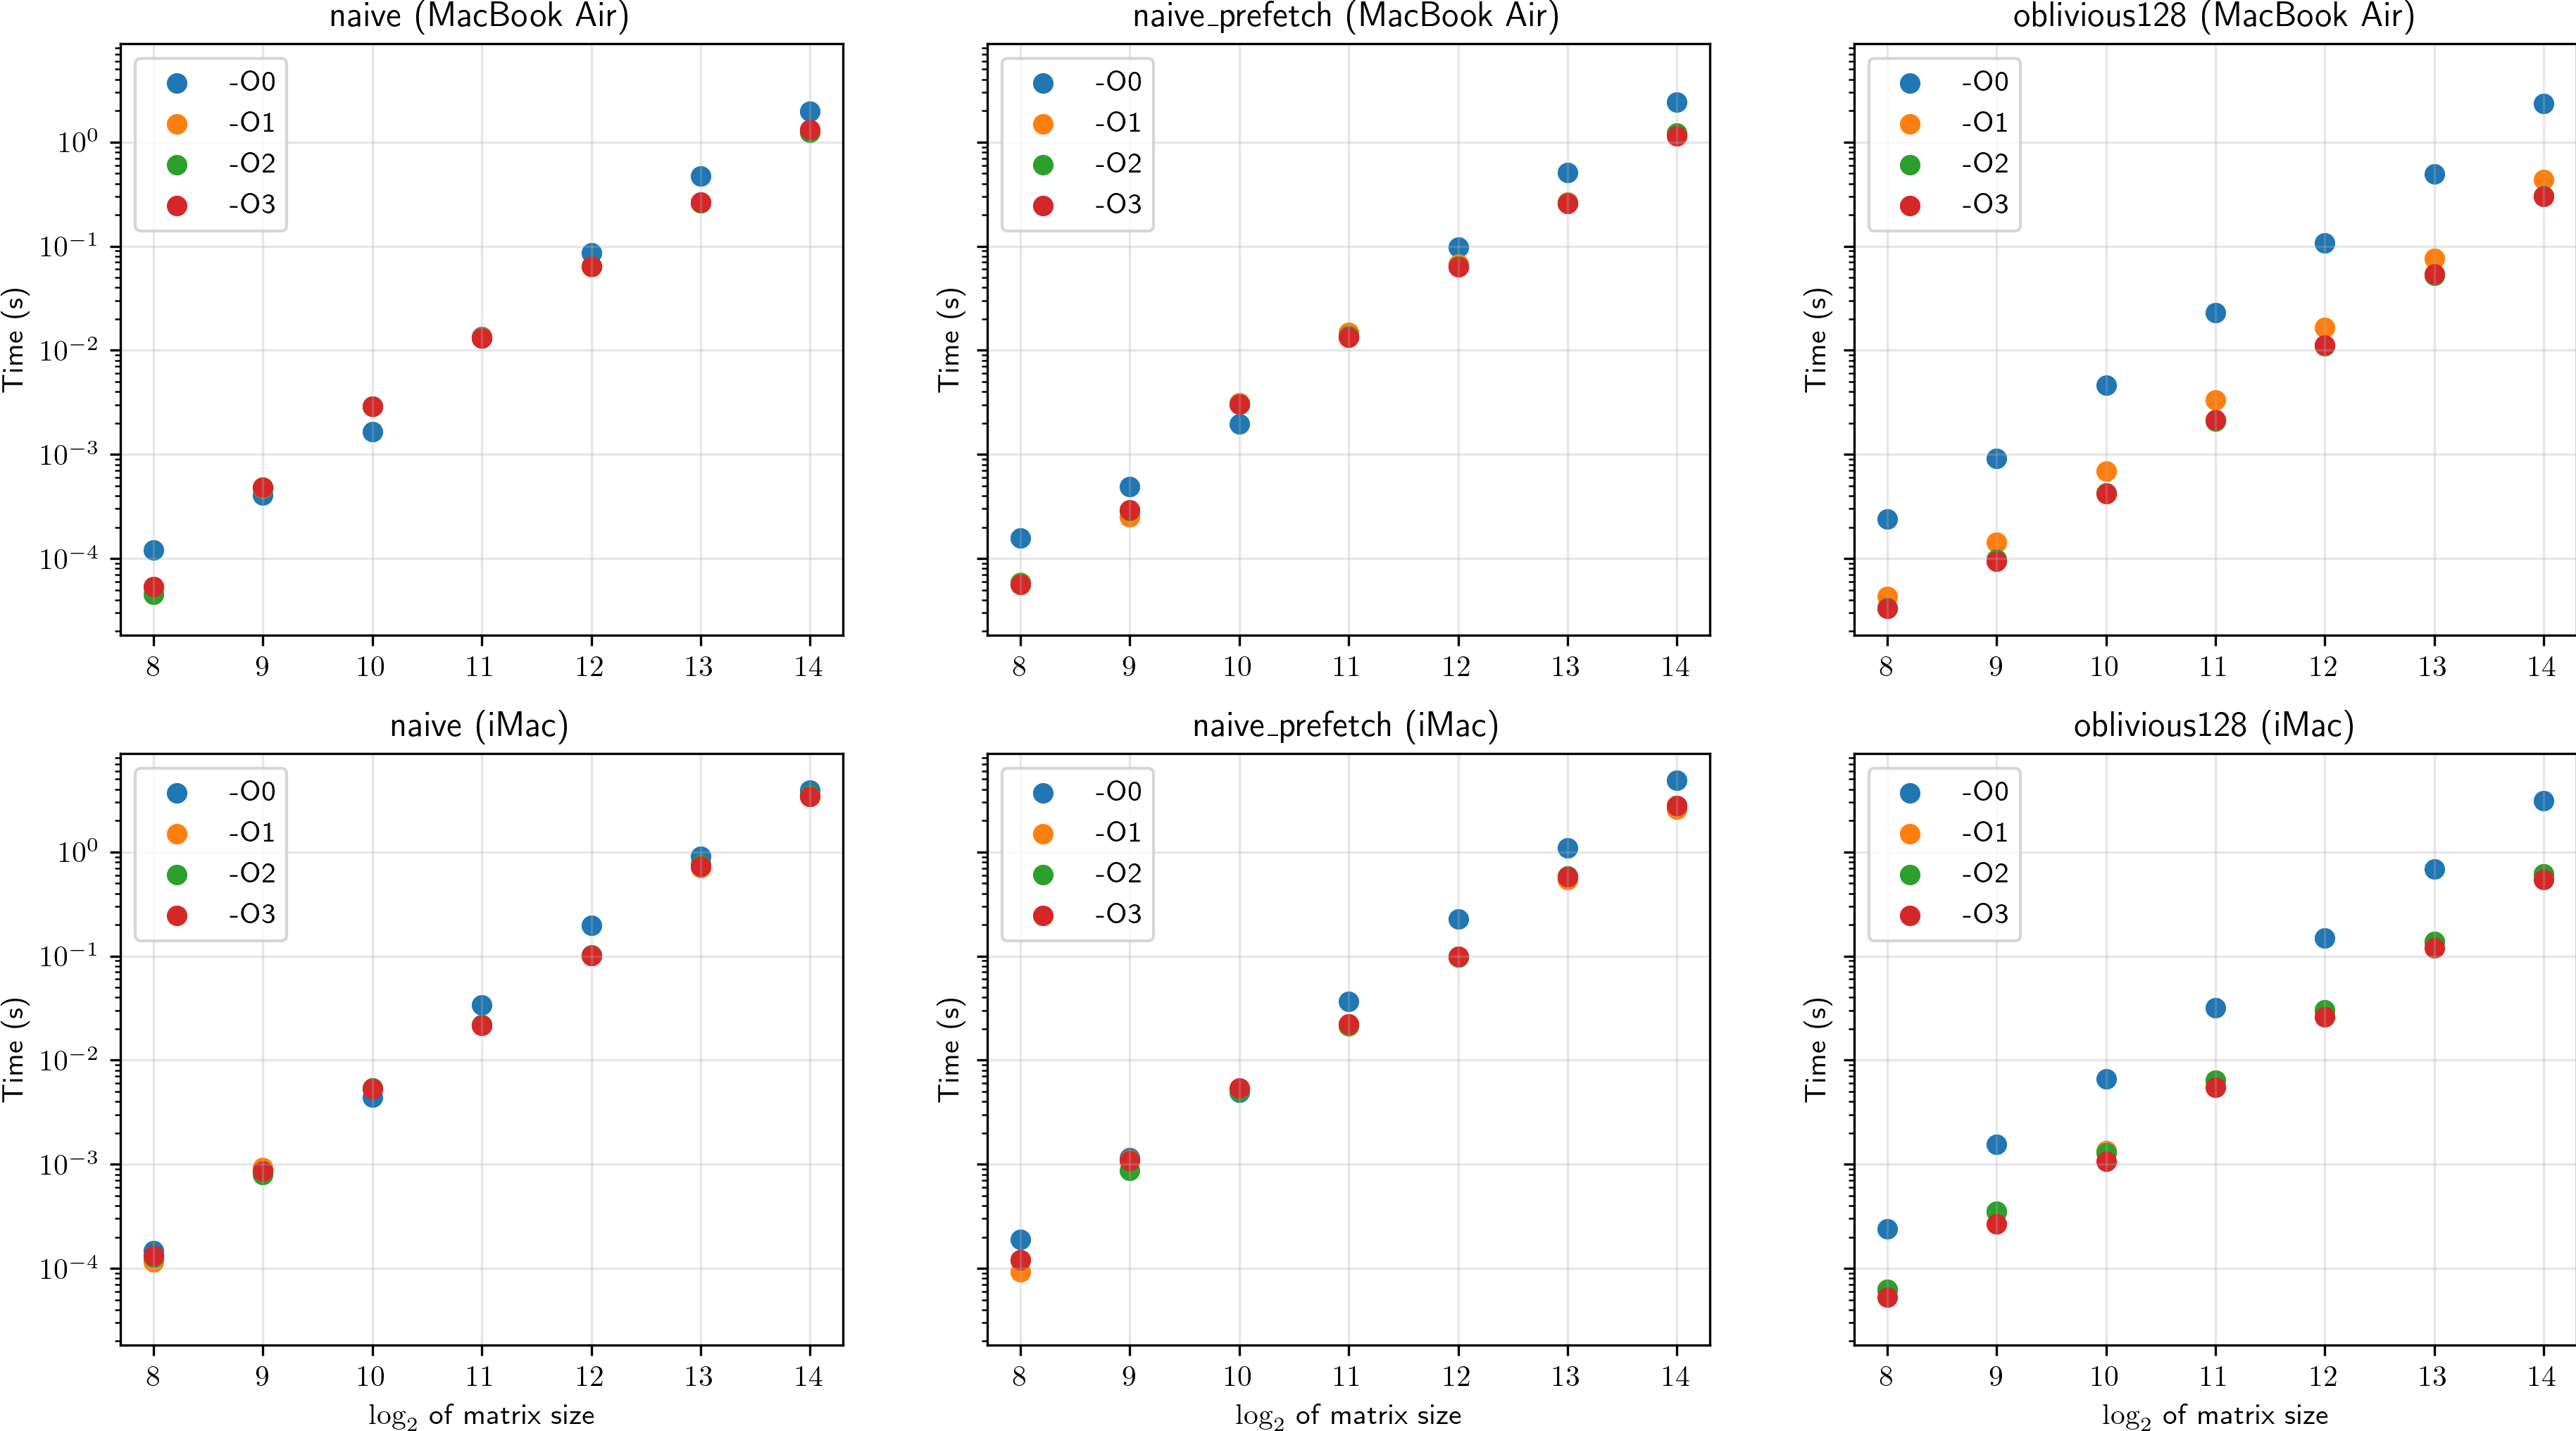
\includegraphics[width=0.7\textwidth]{./images/time_comparision.png}
        \caption{Comparison of the mean execution time of various algorithms for matrix sizes ranging from $2^8$ to $2^{14}$ for the MacBook Air architecture (upper row) and iMac architecture (bottom row). The y-axis denotes the execution time in seconds and is depicted on a logarithmic scale.}
        \label{fig:time_comparison}  
    \end{figure*}

    \begin{figure*}[htbp]
        \centering
        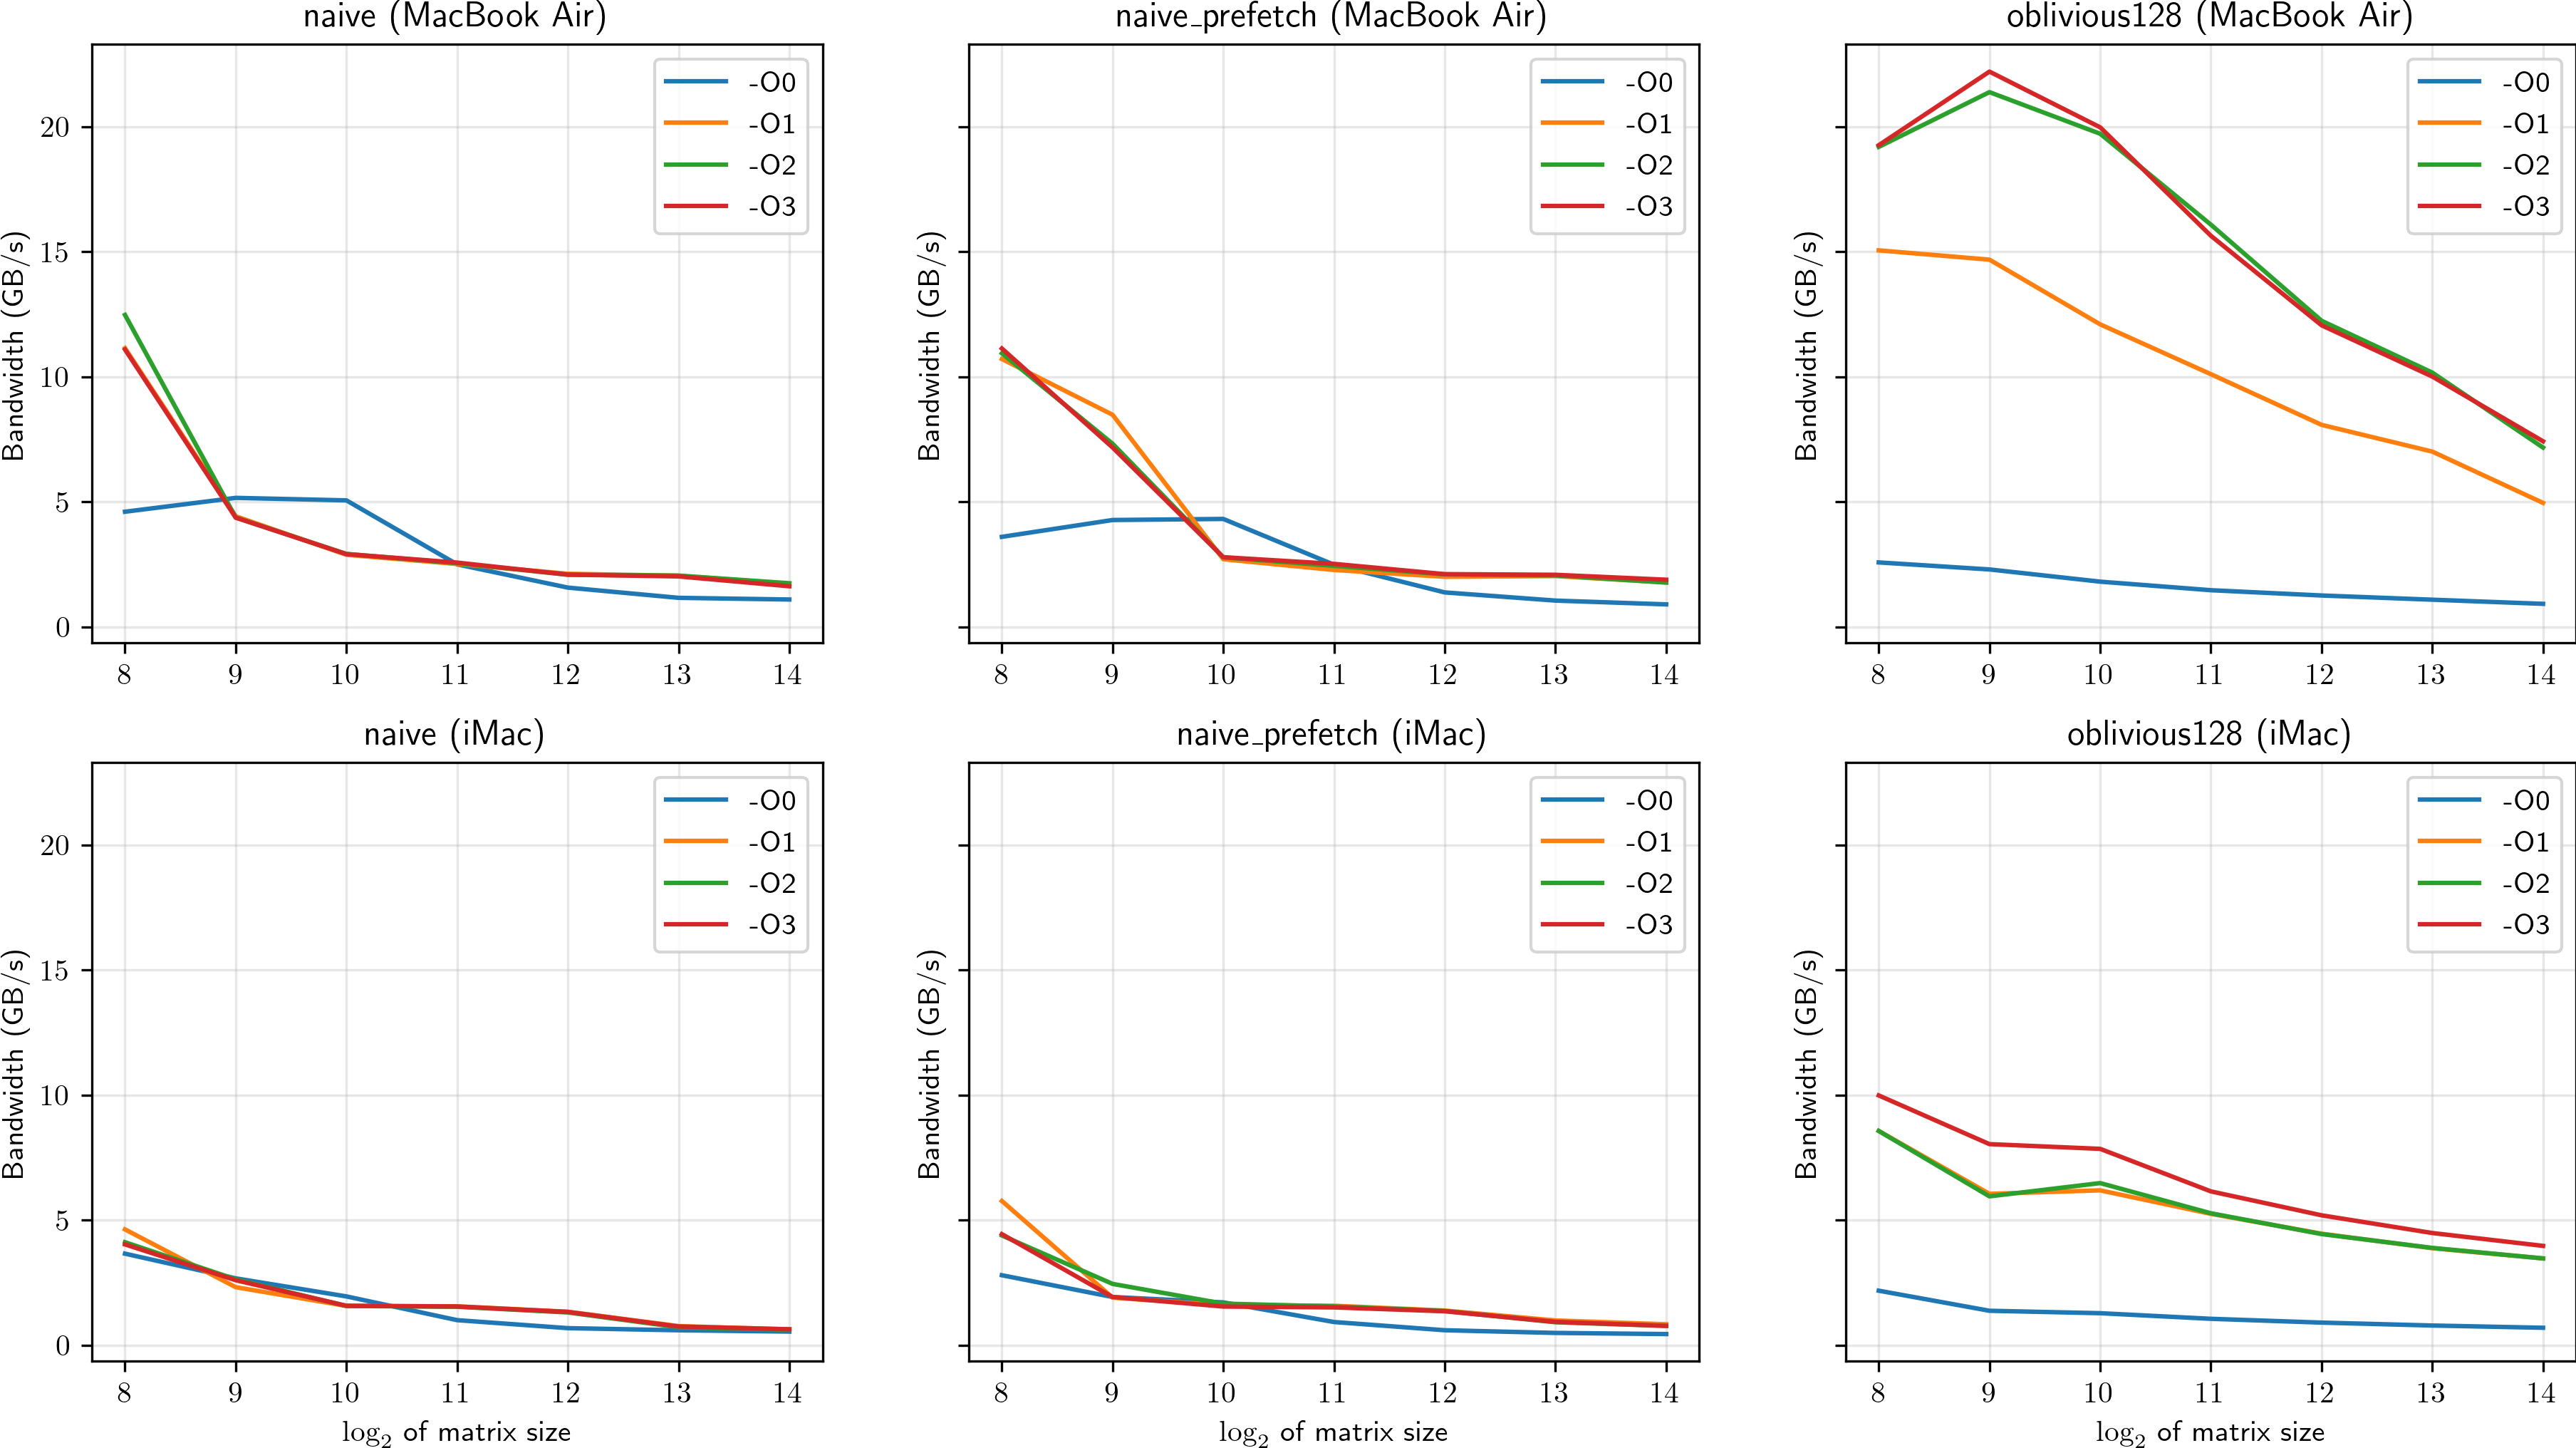
\includegraphics[width=0.7\textwidth]{./images/bandwidth_comparision.png}
        \caption{Comparison of the mean effective bandwidth of different algorithms for matrix sizes between $2^8$ and $2^{14}$ for the MacBook Air architecture (upper row) and iMac architecture (bottom row).}
        \label{fig:bandwidth_comparison}  
    \end{figure*}

    The execution times of the different algorithms are compared in Figure \ref{fig:time_comparison}.
    The third algorithm (\texttt{oblivious128} in Figure \ref{fig:time_comparison}) achieved the highest speedup with optimization flags. It showed a speedup of $7.81$ on the MacBook Air and $5.7$ on the iMac when comparing non-optimized code to code with \texttt{-O3} enabled for matrix size $2^{14}$.
    On the MacBook Air, the third algorithm gained an additional speedup of $1.46$ for matrix size $2^{14}$ using \texttt{-O2} and \texttt{-O3} optimizations compared to \texttt{-O1} optimization.
    The second algorithm (\texttt{naive\_prefetch} in Figure \ref{fig:time_comparison}) performs slightly better for large matrices with some optimization enabled, resulting in a speedup of $2.11$ on the MacBook Air and $1.73$ on the iMac for matrix size $2^{14}$.
    Enabling optimization flags can be disadvantageous for execution time performance (see \texttt{naive} and \texttt{naive\_prefetch} implementations for matrix size $2^{10}$).

    The effective bandwidth of the different algorithms is compared in Figure \ref{fig:bandwidth_comparison}. It's evident across all graphs that the effective bandwidth decreases as the matrix size increases. This trend arises because the matrix size grows exponentially with a base of $2$, while the execution time grows exponentially with a base of roughly $10$, as illustrated in Figure \ref{fig:time_comparison}. Consequently, the execution time increases more rapidly than the matrix size, leading to a decline in effective bandwidth.

    Cache data, as depicted in Figure \ref{tab:cache_data} in the appendix, reveals distinctive behaviors among implementations. Specifically, the \texttt{naive} and \texttt{naive\_prefetch} implementations show similar cache patterns, while the \texttt{oblivious128} implementation stands out with different cache behavior. Comparing cache data across implementations, it's evident that the \texttt{oblivious128} implementation requires approximately twice as many instructions, data reads, and data writes as the \texttt{naive} implementation. The variance could be a result of the extra instructions required for transposing submatrices and copying quadrants in the \texttt{oblivious128} algorithm, leading to a greater overall instruction count. Another notable finding is that the last-level data cache read misses are significantly lower for the \texttt{oblivious128} implementation. This may be due to the improved fit of submatrices utilized in the \texttt{oblivious128} algorithm within the cache.

    \begin{table}[htbp]
        \caption{Summarized cache data for different CPU implementations with \texttt{-O3} optimization}
        \begin{center}
            \begin{tabular}{ | c | c | c | c | c | c | c |}
                \hline  
                Name                    & Ir    & Dr    & DLmr  & Dw    & D1mw  & DLmw \\
                \hline  
                \texttt{naive}          & 20.6  & 5.1   & 0.14  & 2.4   & 0.016 & 0.016\\ 
                \hline  
                \texttt{oblivious128}   & 41.1  & 10.1  & 0.041 & 4.7   & 0.033 & 0.033\\      
                \hline  
            \multicolumn{4}{l}{$^{\mathrm{a}}$Values are given in billions}     
            \end{tabular}       
        \end{center}
        \label{tab:cache_data}
    \end{table}

    \section{GPU Experiments}
    \subsection{Setup}
    For benchmarking the GPU implementations, the following setup was used. Both GPU algorithms were compiled with \texttt{nvcc} of the CUDA 12.5 module provided on the Marzola cluster of the University of Trento. To measure the speedup compared to the CPU implementations, also Algorithm \ref{fig:naive_implementation} and Algorithm \ref{fig:rec_implementation} were compiled using \texttt{-O3} optimizations. Each resulting binary was evaluated 50 times for matrix sizes between $2^8$ and $2^{14}$. CUDA algorithms were also benchmarked with block sizes of 4, 8, 16 and 32. The grid size was computed using the matrix and block size. Time was only measured for the kernel execution, so the time for moving data from and to the GPU device is not contained in the measurements. The experiments were only conducted on the Marzola cluster of the University of Trento, since there was no other possible access to GPUs during the homework. On the cluster an Nvidia A30 GPU, with a theoretical peak bandwidth of 933GB/s was used to benchmark the implementations.

    \subsection{Results}
    \begin{table*}[htbp]
        \caption{Comparison of the mean effective bandwidth for different algorithms by matrix size}
        \begin{center}
            \begin{tabular}{ | c | c | c | c | c | c | c | c |}
                \hline  
                Name                    & $2^8$    & $2^9$    & $2^{10}$  & $2^{11}$    & $2^{12}$  & $2^{13}$ & $2^{14}$ \\
                \hline  
                \texttt{cpu\_oblivious128}& 15.77  & 14.36  & 11.99  & 9.05  & 6.98 & 6.18 & 5.49\\ 
                \hline  
                \texttt{gpu\_naive\_4}& 17.33  & 24.17  & 49.58 & 66.96   & 75.05 & 77.02 & 76.25 \\      
                \hline  
                \texttt{gpu\_naive\_16}& 23.16  & 31.60  & 98.01 & 225.78   & 209.64 & 228.44 & 307.66 \\      
                \hline  
                \texttt{gpu\_naive\_32}& 19.27  & 27.57  & 72.19 & 120.98   & 137.47 & 148.41 & 142.33 \\      
                \hline  
                \texttt{gpu\_tiled\_4}& 17.69  & 24.60  & 52.08 & 71.55   & 76.06 & 76.67 & 77.14\\      
                \hline  
                \texttt{gpu\_tiled\_16}& 23.74  & 39.72  & 128.99 & 311.84   & 437.74 & 500.53 & 517.83\\      
                \hline  
                \texttt{gpu\_tiled\_32}& 22.65  & 35.09  & 115.23 & 309.69   & 403.84 & 451.99 & 471.01\\      
                \hline  
            \multicolumn{4}{l}{$^{\mathrm{a}}$Values are given in GB/s}     
            \end{tabular}       
        \end{center}
        \label{tab:gpu_bandwidth}
    \end{table*}
    \begin{figure}[htbp]
        \centering
        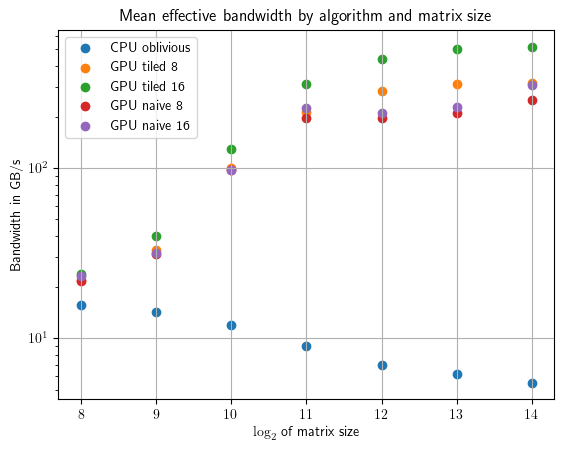
\includegraphics[width=0.4\textwidth]{./images/gpu_bandwidth.png}
        \caption{Comparison of mean effective bandwidth for different algorithms and matrix sizes}
        \label{fig:gpu_bandwidth}  
    \end{figure}
    \begin{figure}[htbp]
        \centering
        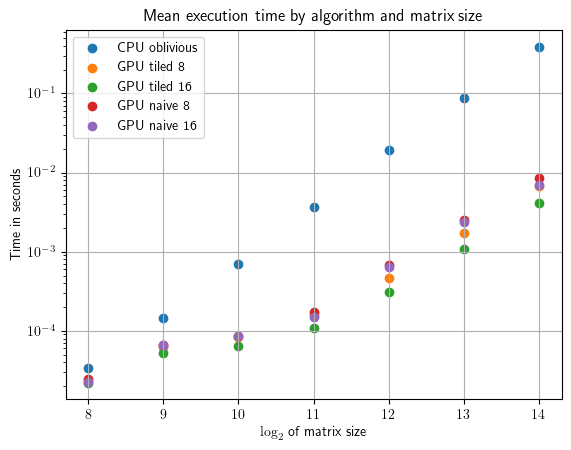
\includegraphics[width=0.4\textwidth]{./images/gpu_time.png}
        \caption{Comparison of mean execution time for different algorithms and matrix sizes}
        \label{fig:gpu_time}  
    \end{figure}
    The results obtained during the experiments are summarized in Table \ref{tab:gpu_bandwidth} and depicted in Figure \ref{fig:gpu_bandwidth} and Figure \ref{fig:gpu_time}. Note that the label \texttt{gpu\_tiled\_16} stands for the tiled GPU algorithm (Algorithm \ref{fig:cuda_tiled_implementation}) with a block size of 16. One can make multiple observations from the data. The most obvious observation is that GPU algorithms perform significantly better than the CPU algorithms. In every scenario, the GPU algorithms have a higher effective bandwidth, compared to the CPU algorithms. In the best case, the effective bandwidth of the \texttt{gpu\_tiled\_16} algorithm is 94 times higher compared to the CPU algorithm. 
    The second observation is that while the effective bandwidth decreases as matrix size increases for CPU algorithms, the effective bandwidth for GPU algorithms increases for bigger matrices.
    The third observation is that the difference in performance between \texttt{gpu\_naive} (Algorithm \ref{fig:cuda_naive_implementation}) and \texttt{gpu\_tiled} (Algorithm \ref{fig:cuda_tiled_implementation}) is quite small for smaller matrices, but grows as the matrix size increases. That means that for larger matrices, the usage of shared memory has a bigger effect on performance. The fourth observation is that the block size does affect the performance. In the experiments the optimal performance was achieved by using a block size of 16. Increasing the block size to 32 caused a drop in effective bandwidth for all GPU algorithms and matrix sizes.

    \section{Conclusion}
    After analyzing various algorithms and metrics, it's evident that utilizing blocks can enhance the performance of matrix transposition algorithms. This was demonstrated through the better execution time and effective bandwidth of compiler-optimized versions of the \texttt{oblivious128} implementation, which incorporates a form of blocking. The third algorithm also presents promising directions for parallelization, as each submatrix can be processed independently, offering straightforward potential for parallel execution.

    The main observation made during the homework was the significant increase in performance by using GPU acceleration. Using GPUs for parallelization can result in large improvements with respect to effective bandwidth and execution time. It was also observed that a careful design of the GPU algorithm is needed. Different implementations and parameter choices can result in significant performance differences, even if the algorithm is executed on a GPU. The presented CUDA kernels could be further improved by using more advanced features of the CUDA platform, such as multiple streaming processors. Another approach could be to finetune the parameter choices. In the presented experiments, a block size of 16 was optimal, but further parameter choices could be investigated. One could also optimize the CUDA implementation to run on multiple GPUs. 

    \newpage
    \printbibliography

\end{document}